\documentclass[a4paper]{article}

\usepackage[danish,english]{babel}
\usepackage[utf8]{inputenc}
\usepackage{amsmath}
\usepackage{rotating}
\usepackage{float}
\usepackage{subfig}
\usepackage{graphicx}
\graphicspath{{./graphics/}} 
\usepackage[colorinlistoftodos]{todonotes}
\newcommand{\namedtodo}[5]
{
  \ifthenelse{\equal{#1}{}}
  {
    \todo[backgroundcolor=#4,linecolor=#4,caption=
    {\textbf{#3: } #2}]
    {\color{#5}\textbf{#3: }#2}
  }
  {
    \todo[backgroundcolor=#4,linecolor=#4,caption=
    {\textbf{#3: } #1}]
    {\color{#5}\textbf{#3: }#2}
  }
}
\newcommand{\namedtodoinline}[5]
{
  \ifthenelse{\equal{#1}{}}
  {
    \todo[backgroundcolor=#4,caption=
    {\textbf{#3: } #2}
    ,inline]
    {\normalsize\color{#5}\textbf{#3: }#2}
  }
  {
    \todo[backgroundcolor=#4,caption=
    {\textbf{#3: } #1}
    ,inline]
    {\normalsize\color{#5}\textbf{#3: }#2}
  }
}
\newcommand{\mikkel}[2][]{\namedtodo{#1}{#2}{Mikkel}{blue!80}{white}}
\newcommand{\stefan}[2][]{\namedtodo{#1}{#2}{Stefan M}{orange}{black}}
\newcommand{\mikael}[2][]{\namedtodo{#1}{#2}{Mikael}{green}{black}}
\newcommand{\bruno}[2][]{\namedtodo{#1}{#2}{Bruno}{black!10!red!90}{white}}
\newcommand{\ivan}[2][]{\namedtodo{#1}{#2}{Ivan}{white!10!purple!90}{black}}

\makeatletter \renewcommand \listoftodos{\section*{List of Todos} \@starttoc{tdo}\clearpage}
\usepackage[backend=bibtex,
  bibencoding=utf8,natbib
  ]{biblatex}
\addbibresource{bib}
\usepackage[colorlinks=true,allcolors={black}]{hyperref}
\usepackage[danish]{cleveref}


\title{SharePass - Sikre passwords og sikker deling af passwords og licenser for virksomheder}

\author{Stefan Marstrand Getreuer Micheelsen \and Mikael Elkiær Christensen \and Mikkel Sandø Larsen \and Bruno Thalmann}

\date{\today}

\begin{document}
\maketitle
\listoftodos

\section{Idé}
Dette afsnit vil indføre læseren i vores ide hvilket vil gøre det lettere at følge resten af rapportens indhold.
Først vil ideen blive præsenteret uformelt for derefter at blive præsenteret gennem storytelling.

Vi ønsker at udvilke en password manager med deling for firmaer og private

Det primære produkt er et NFC kort der lagrer krypterede passwords.
Dette kort skal bruges i alle login der udføres i en virksomhed, det vil sige både fysisk indgang til bygningen, login til computere, login i programmer samt licenser til produkter som word og matlab.

Det hele kobles sammen af en lokal central der indeholder alle passwords.
Ved brug af kortet synkroniseres dette samtidig.
Dette betyder at al administrering af koder kan styres, og medarbejderen skal derfor ikke tænke over hverken kodestyrke eller fornyelse af kode.
Ligeså snart der er en ny kode der skal benyttes i en arbejdsgang vil denne blive synkroniseret.

\subsection{Design - Storytelling}
Dette afsnit præsenterer den teknik vi har benyttet i forbindelse med designet af vores business model - storytelling.
Beskrivelsen af storytelling er baseret på \citet[p.~125]{osterwalder2009business}
Storytelling går ud på at undersøge forskellige business models igennem en historie der beskriver hvordan produktet skal fungere.
Denne historie kan præsenteres på flere måder.
Man kan bruge illustrationer som udgangspunkt til en diskussion om produktet, man kan lave en videopræsentation der præsenterer hvordan produktet skal fungere eller man kan lave en tegneserie der beskriver hvordan interaktion med produktet skal forløbe.
Storytelling har til formål at gøre et koncept mere håndgribeligt så det er lettere at diskutere og derved lettere at udvikle sin business model.

Vi har valgt at lave en tegneserier der beskriver først den nuværende situation og derefter hvordan vi forestiller os at forbedre situationen med vores produkt.
I \cref{story:badpass:boss} og \cref{story:sharing} præsenteres de potentielle problemstillinger der afhjælpes ved brug af SharePass.

I \cref{story:badpass} anvender en virksomheds medarbejdere dårlige\footnote{Eksempelvis meget korte eller almindeligt brugte adgangskoder.} adgangskoder.
I \cref{story:sharing} deles adgangskoder (eksempelvis for nye medarbejdere) via email.
Alternativt ville denne deling også kunne ske på papir ved at ophænge \emph{fælles} adgangskoder i kontorer.

Problemerne afhjælpes i \cref{story:sharepass} med SharePass.
Her får virksomhedens direktør et system der løser ovenstående problemer ved automatisk at generere nye adgangskoder for systemets medarbejdere og lade disse blive anvendt ved hjælp af elektroniske identifikations-kort.

{
% Command and settings for creating the storytelling comics
\newcommand{\storyfig}[1]{\fbox{\includegraphics[height=5cm]{graphics/story_#1}}}
\setlength\fboxsep{0pt}
\setlength{\fboxrule}{1pt}

\begin{sidewaysfigure}
\centering
\subfloat[En virksomhed bestående af direktør Steen og hans to ansatte Anders og Birte.]
{\storyfig{01}\label{story:badpass:init}} \quad
\subfloat[Anders og Birte tilgår services ved hjælp af deres adgangskoder \emph{abc} og \emph{1234}.]
{\storyfig{03}\label{story:badpass:pass}} \quad
\subfloat[Steen er bekymret for beskyttelsen af virksomhedens oplysninger på grund af medarbejdernes valg af koder.]
{\storyfig{04}\label{story:badpass:boss}}
\caption{Medarbejdere anvender dårlige adgangskoder}\label{story:badpass}
\end{sidewaysfigure}

\begin{sidewaysfigure}
\centering
\subfloat[En virksomhed bestående af direktør Steen og hans to ansatte Anders og Birte.]
{\storyfig{01}\label{story:sharing:init}} \quad
\subfloat[Anders mangler adgang til en applikation og Birte sender derfor den fælles adgangskode til Anders via email.]{\storyfig{07}\label{story:sharing:pass}} \quad
\subfloat[Steen er bekymret for beskyttelsen af virksomhedens adgangskoder på grund af medarbejdernes delings-metode.]
{\storyfig{05}\label{story:sharing:boss}}
\caption{Deling af adgangskoder foregår åbent og ukrypteret.}\label{story:sharing}
\end{sidewaysfigure}

\begin{sidewaysfigure}
\centering
\subfloat[Anders og Birte får hver udleveret et personligt identifikations-kort med en NFC chip.]
{\storyfig{08}\label{story:sharepass:nfc}} \quad
\subfloat[De koder Anders og Birte anvender er ikke længere selvbestemt.
Der anvendes derfor længere og ikke almindelige adgangskoder.]
{\storyfig{09}\label{story:sharepass:login}}\\
\subfloat[Adgangskoder administreres af en central server og deles elektronisk med medarbejdernes kort.
Ændring af adgangskoder og tildeling af licenser/koder til en medarbejder administrerers af det centrale system.]
{\storyfig{11}\label{story:sharepass:server}} \quad
\subfloat[Steen er tilfreds da han nu har mulighed for, via det centrale system, at administrere Anders og Birtes licenser og er sikret at adgangskoderne er lange.]
{\storyfig{10}\label{story:sharepass:success}}
\caption{Brug af SharePass sikrer at Steens medarbejdere anvender bedre\\ adgangskoder og administrerer deling blandt medarbejderne.}\label{story:sharepass}
\end{sidewaysfigure}
}

\section{Værdiskabelse}
For at være bæredygtig på markedet er det vigtigt at vide hvilke styrker og svagheder ens firma har.
\citep[p.~11]{rose2012software} præsenterer teorier fra entreprenørskab der kan beskrive hvordan firmaer skaber værdi på et marked.
Et udpluk af disse teorier vil her blive gennemgået for at have et godt fundament inden der skabes en konkret business model.

\subsection{Value chain}\label{value_chain}


Porter's value chain model beskriver et firma ud fra de aktiviteter der skal udføres for at tilføje værdi til de ``rå'' materialer.
Eftersom modellen er konstrueret med konventionelle fremstillingsvirksomheder i tankerne kan det ikke direkte overføres til softwarevirksomheder.
Softwarevirksomheder indkøber sjældent rå materialer i traditionel forstand, men ideerne gælder stadig på et konceptuelt niveau.
Følgendende beskrivelse er baseret på \citet[p.~12]{rose2012software}.


Aktiviteter inddeles i to kategorier, de primære og support aktiviteter.
De primære aktiviteter beskriver hvordan virksomheden omdanner rå materialer til det færdige produkt på hylden ved at tilføje værdi.
Support aktiviteterne bidrager til denne omdannelse uden direkte at tilføre værdi, dette kan eksempelvis være research.
Modellen er illustreret på  \cref{valuechain}.

\begin{figure}[H]
	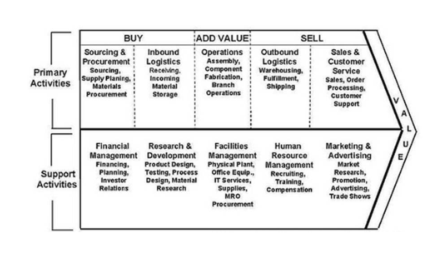
\includegraphics[width=\textwidth]{valuechain.PNG}
	\caption{Porters valuechain model}
	\label{valuechain}
\end{figure}

\paragraph{Model af SharePass}
Følgende er en valuechain model af SharePass virksomheden.
De primære aktiviteter består i at indkøbe de hardwaredele som vi ikke selv kan stå for at producere.
Vi tilføjer derefter værdi til disse ved at designe sikkerhedsprotokoller til enhederne samt software til klient og server.
Værdien består primært i at lave en løsning der virker med et minimum af interaktion men stadig sikkert.
Salgsdelen går derefter ud på at sælge produktet til virksomheder og derefter yde support så de får mest muligt ud af produktet.

Til at muliggøre de primære aktiviteter benyttes supportaktiviteterne.
For at sikre den højst mulige sikkerhed er det nødvendigt at hyre eksperter i sikkerhed.
Ligeledes har vi brug for ekspertise inden for udvikling af hardwaredelen af produktet.
Der skal derfor også hyres eksperter inden for elektronik og hardware samt koblingen mellem elektronikken og software systemet.
For at få produktet solgt er det vigtigt at henvende sig til virksomheder på en måde der kan overbevise dem om hvorvidt de har et behov for produktet.
Til dette skal der bruges en marketingafdeling.

\paragraph{SharePass' valuechain}
\subparagraph*{Primære aktiviteter}
\subparagraph*{} 
Køb:
\begin{itemize}
\item NFC kort
\item Fysisk login med NFC kort hos firma - her opdateres passwords på kortet
\end{itemize}
Tilføj værdi:
\begin{itemize}
\item Sikkerhedsprotokol mellem fysisk login portal og server
\item Sikkerhedsprotokol mellem klient og NFC kort
\item Sikkerhedsprotokol mellem fysisk login portal og NFC kort
\item Software til password server
\item Software til klient
\end{itemize}
Sælg:
\begin{itemize}
\item Sælg produkt som pakke
\item Tilbyd support
\end{itemize}

\subparagraph*{Support aktiviteter}
\begin{itemize}
\item Marketing
\item Hyre - sikkerhedsekspert, hardwaredesigner
\end{itemize}

Denne teori beskæftiger sig med hvad et firma formår på baggrund af dets ressourcer, \citet[p.~12]{rose2012software}.
Ressource i denne kontekst er et vidt begreb som kan ses på \cref{rbt_fig}, her kan man også se det mulige formåen.

\begin{figure}[H]
  \begin{center}
    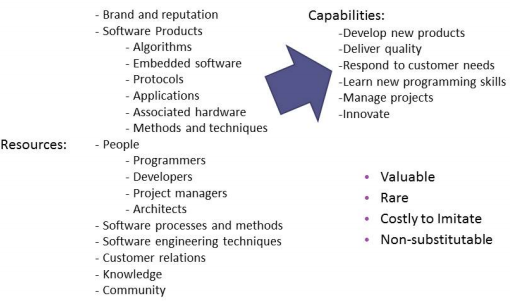
\includegraphics[width=.8\textwidth]{resource_based_theory.png}
  \end{center}
  \caption{Et eksempel på ressourcer og mulig formåen i Resource Based Theory.}
  \label{rbt_fig}
\end{figure}

\paragraph{Ressourcer:}
Denne paragraf lister de ressourcer vores virksomhed har til rådlighed:
\begin{itemize}
\item Team:
  \begin{itemize}
  \item Programmør
  \item Sikkerhedsekspert(konsulent)
  \item Hardwaredesigner
  \item Sælger
  \item Systemarkitekt
  \item Usability(konsulentfirma)
  \end{itemize}
\item Produkter
  \begin{itemize}
  \item NFC kort
  \item Fysisk login portal
  \item Software klient - ansattes pc kommunikation med NFC kort
  \item Server sofware - deling og håndtering af passwords og licenser
  \item Sikkerhedsprotokol mellem fysisk login portal og server
  \item Sikkerhedsprotokol mellem klient og NFC kort
  \item Sikkerhedsprotokol mellem fysisk login portal og NFC kort
  \end{itemize}
\item Pakkeløsning
\item Kundeservice
  \begin{itemize}
  \item Opsætning
  \item Udvidelse
  \item Support
  \end{itemize}
\item Viden om:
  \begin{itemize}
  \item Sikkerhed
  \item Kunders(virksomheder) workflow
  \item Softwarearkitektur
  \end{itemize}
\item Demo setup - som kan bruges til fremføring og test
\end{itemize}
\paragraph{Beskrivelse af team}
Vores team består af os selv, fire mand som står for:
\begin{itemize}
\item Systemarkitektur(hardware og software)
\item Til dels sikkerhed
\item Software
\item Support
\end{itemize}
Udover det består det af en sælger, en hardwaredesigner, en sikkerhedskonsulent og et konsulentfirma til evaluering af usability af produktet.
\paragraph{Formåen:}
Det giver os en mulighed for at levere en samlet løsning, skræddersyet til kunden som er sikker at bruge.
Det er en løsning hvor der satses på god usability, og at det ikke forstyrrer de ansattes i deres daglidag, ved fx at ændre deres workflow.
De ansatte skal ikke tænke på sikkerhed men data er alligevel beskyttet af sikre passwords.


\subsection{Five forces}
 Porter præsenterer også en alternativ måde at forstå et startups succes, kaldet "Five forces".
 Disse "five forces" beskriver den konkurrencekontekst som virksomheden indgår i.
 Følgende beskrivelse er baseret på \citet[p.~16]{rose2012software}.

 Ifølge Porter er succesen af et startup delvis defineret af hvordan virksomheden konkurrerer med andre virksomheder på samme marked.
 Porters model kan ses på \cref{fiveforces}.

\begin{figure}[H]
	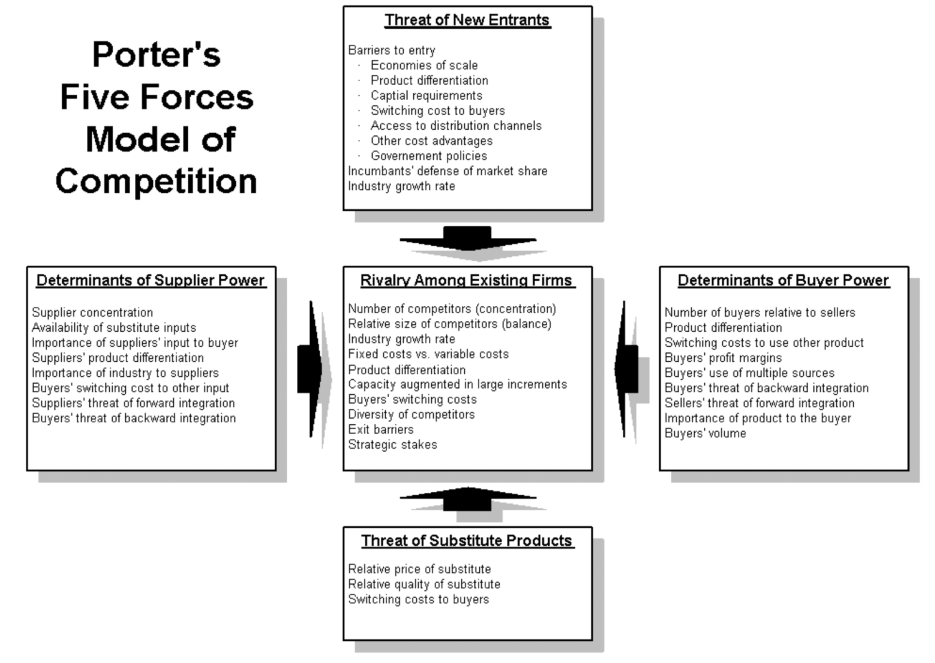
\includegraphics[width=\textwidth]{fiveforces.PNG}
	\caption{Five forces modellen}
	\label{fiveforces}
\end{figure}

\paragraph{Five Forces i SharePass' marked}
\label{par:five_forces_i_sharepass_marked}

For at beskrive det marked SharePass skal konkurrere benyttes Five Forces modellen. 
Hver af de fem markedskræfter er beskrevet med de mest karakteriserende elementer.
Det engelske udtryk ``switching cost'' er brugt i denne kontekst til at beskrive det en kunde skal ændre for at gå fra et produkt til et andet.

\begin{description}
	\item[Rivalry among existing firms] Der findes mange password managers, både ren software og hardware managers. Typisk benyttes en abonnementsmodel.
	\item[Threat of new entrants] Vores produkt har en væsentlig "switching cost" i forhold til eksisterende løsninger (der dog ikke er lige så integreret i virksomheden). 
	\item [Threat of substitute products] Vores produkt kan få konkurrence af mindre avancerede løsninger der har lavere "switching cost".
	\item [Determinants of Supplier Power] Vores hardware er ikke specific for en supplier og det er derfor let at skifte. 
	\item [Determinants of Buyer Power] Fokus er at skræddersy til virksomheder hvilket betyder at virksomhederne har en stor magt.
\end{description}
\stefan{Vi skal nok lige kigge dem igennem, specielt determinants of s og determinants of b}

\section{Business model}
\begin{figure}
  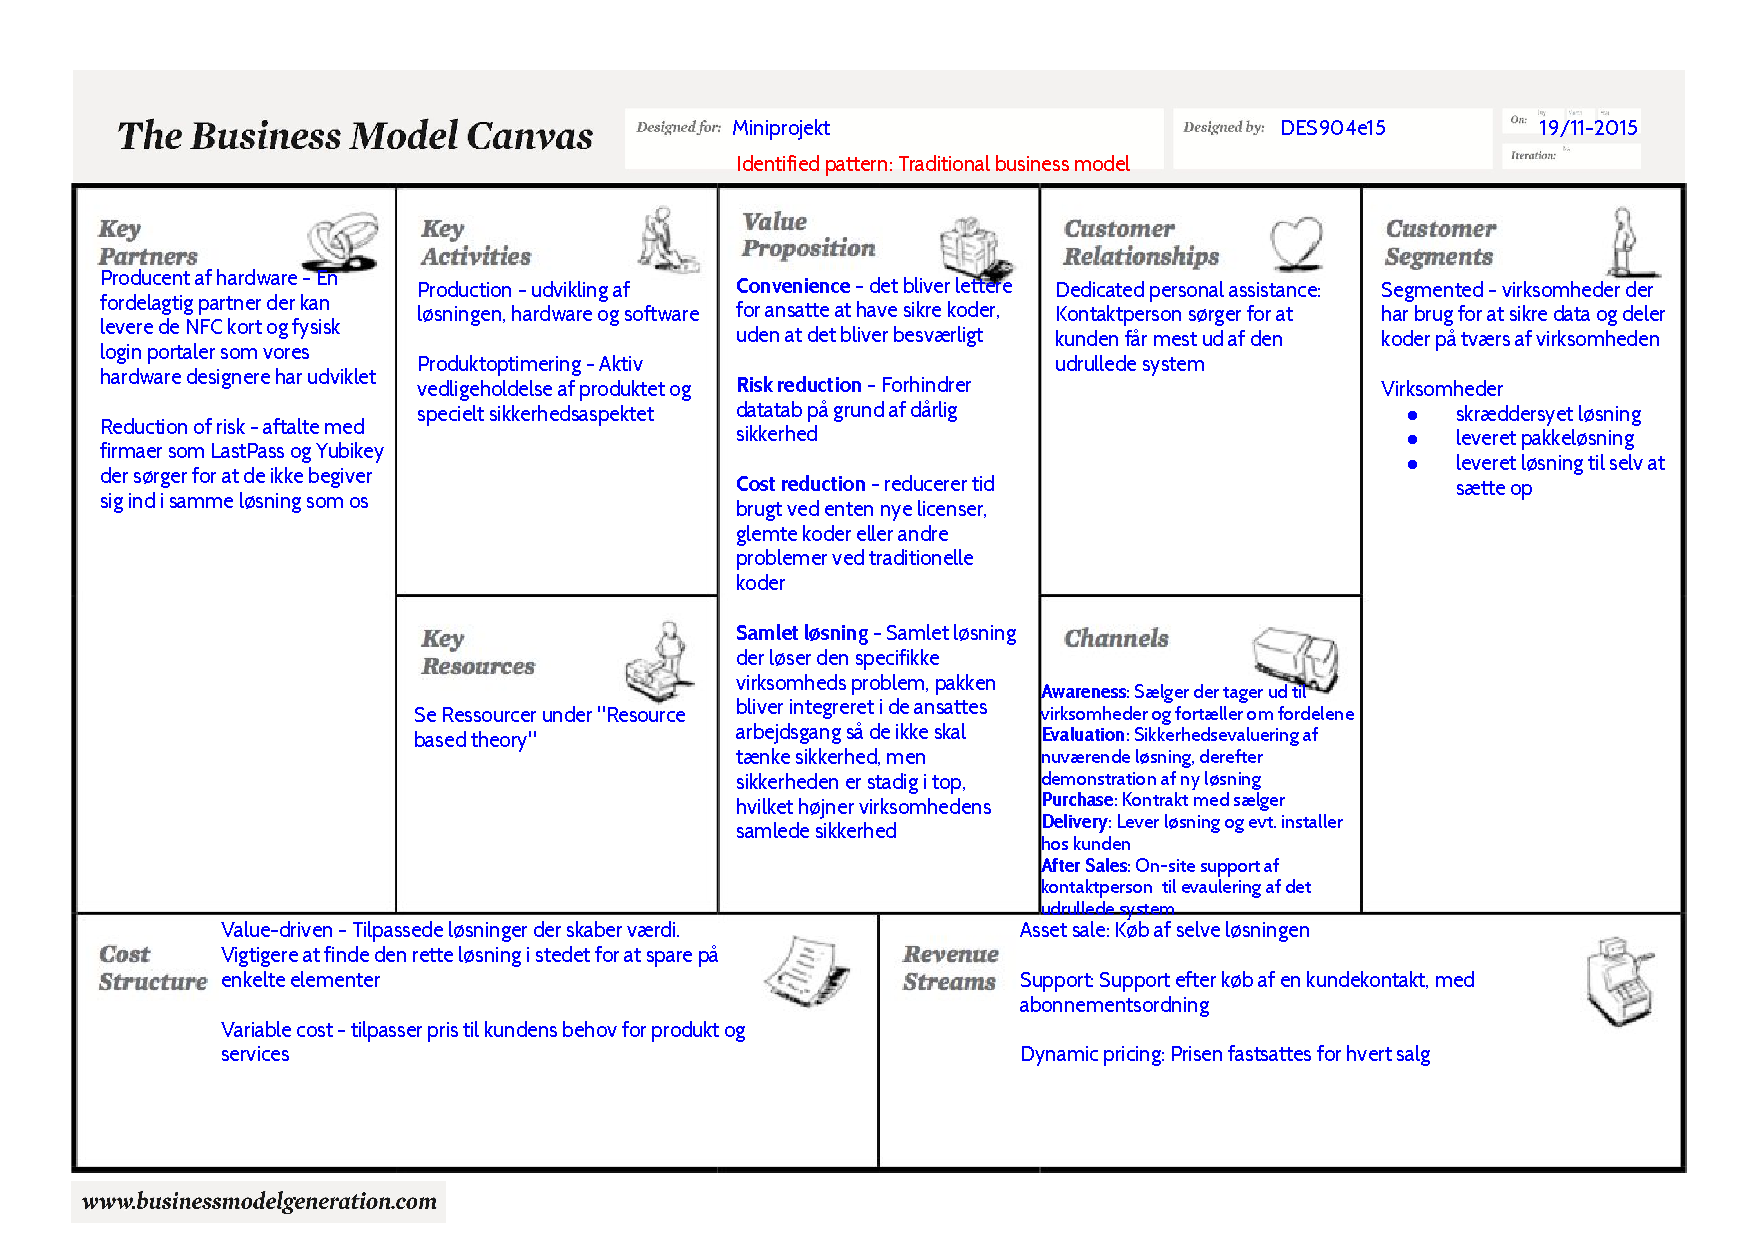
\includegraphics[angle=90, height=0.95\textheight]{graphics/BM.pdf}
  \caption{Business Model Canvas.}
  \label{bm}
\end{figure}

Nu hvor idéen er afklaret og vi har afklaret hvordan vi vil skabe værdi kan vi begynde at designe en business model.
Vi har brugt Business Model Canvas (BMC) fra \citet{osterwalder2009business} til at komme frem til vores business model.
BMC kan bruges til at beskrive, designe, diskutere, udfordre, forbedre og udvikle en BM.
Det er derfor et effektivt værktøj når man er et team med mange forskellige idéer, da det giver et grundlag for bearbejdningen af disse.


BMC består af ni elementer som er med til at sikre at man inkluderer alle væsentlige aspekter af en BM.
Det betyder at man har en liste/skema der kan gennemgås når man ønsker at definere eller bedre en BM.
De ni elementer er: \textit{Customer Segments, Value Propositions, Channels, Customer Relationships, Revenue Streams, Key Resources, Key Activities, Key Partnerships, Cost Structure}.
Vores første BM kan ses på \cref{bm} på side \pageref{bm}.
	

%!TEX root = ../master.tex
\subsection{Faser i Business Model Design Processen}
\citet[pp. 244-259]{osterwalder2009business} foreslår en anvendelig proces til udarbejdning af en ny BM.
Her beskrives 5 faser: \emph{Mobilize, Understand, Design, Implement og Manage}.
Hver af disse faser består af en række aktiviteter der kan udføres for at opnå målene for de enkelte faser.
Undervejs vil der blive både udarbejdet og indført en BM, som til sidst vil blive vedligeholdt.

Den overordnede idé med denne tilgang er at forenkle den ellers komplicerede process; at udarbejde en BM.
Når først en BM er udarbejdet ved denne process er den nem at følge.
Dette er en design-orienteret tilgang, i modsætning til en beslutnings-orienteret tilgang som siger at det er nemt at finde på idéer og problemet i stedet ligger i at vælge en af disse.

For at lave en (ny) BM for vores forretning, har vi fulgt de fem faser fra \citet[pp. 244-259]{osterwalder2009business}.
For hver fase har vi valgt de aktiviteter vi mener er relevante at nævne ifm. udviklingen af vores BM.
Vi har valgt ikke at diskutere faserne ``Implement'' og ``Manage'' da produktet stadig er i et tidligt stadie.
Hvis business modellen udføres er disse to faser nødvendige at udspecificere.

\subsubsection{Mobilize}
\paragraph{Test preliminary business ideas}
Vores BM diskuteres internt, på tværs af hele organisationen, da denne ikke er så stor.
Det er vigtigt at udviklere, sikkerhedsekspert, usability-ekspert og sælgere har en fælles forståelse og enighed omkring forretningens BM.

\paragraph{Assemble team}
Som blev nævnt i \cref{value_chain} og \cref{resource-based} er der samlet et hold.
Dette hold er alsidigt, således at en grundig evaluering af de initielle BMs kan foretages.
Her er det muligt for ethvert medlem af forretningen at bruge deres område/ekspertise til at evaluere de enkelte dele af forretningens BM.

\paragraph{Find lokaler}
For at kunne demonstrere produktet overfor kunder er det nødvendigt at kunne fremvise produktet i en kontekst der tilnærmer sig virkeligheden.
Det er derfor vigtigt at finde lokaler der tillader opsætning af en sådan demonstration.

\subsubsection{Understanding}
\paragraph{Study potential customers}
Vi vil undersøge vores potentielle kunder (virksomheder) og den måde hvorpå de håndterer adgangskoder og licenser.
Herved ønsker vi at opnå en forståelse for hvilke sikkerhedsprotokoller, om nogle, de har og i så fald hvordan de indkorporeres i deres arbejdsproces.
Det er også vigtigt at vi fra starten af virker professionelle, så vi kan opbygge en tillid til disse potentielle kunder.
Da vi beskæftiger os med sikkerhed er dette et særligt vigtigt og følsomt område.

\paragraph{Research already tried}
Her kunne vi kigge på eksisterende løsninger (e.g. LastPass, 1Password) og se hvad de har gjort for at blive udbredte indenfor et marked der minder om vores eget.

\subsubsection{Design}
\paragraph{Prototype}
Vi forestiller os et usability laboratorie i vores egen bygning, som skal afspejle den løsning vi vil give vores kunder.
Det vil sige, at vi har brug for et eller flere rum hvor vores løsning anvendes for at få adgang til rummene.
I de rum skal også være det system der skal bruges til at logge på, samt håndtere centralisering og deling af passwords.

\paragraph{Brainstormet og testet BMs}
For at få testet vores BMs udefra vil vi konsultere os med dem vi mener der ved mest indenfor skabelsen af BMs: Borean Innovation, SEA eller en anden venture capital investor).

%!TEX root = ../master.tex
\subsection{Karakteriser og diskuter value proposition}

Denne sektion vil diskutere den value proposition der blev præsenteret i business modellen på \cref{bm} i et bredt perspektiv.
Diskussionen vil tage udgangspunkt i koncepterne præsenteret i \citet[p.~40]{rose2012software}.

\subsubsection{Type af entreprenør}
Giarratanas tre typer af entreprenør er beskrevet som følger

\begin{description}
	\item[Innovator] Skaber nye produkter der ikke er set før
	\item [Arbitrageur] Udnytter ineffektivitet i markedet. For eksempel kan nuværende løsninger være for dyre eller for besværlige for en bestemt kundegruppe
	\item [Coordinator] Udnytter ressourcer på en alternativ måde
\end{description}

Af disse typer er vores virksomhed en arbitrageur.
Vi bringer noget nyt til markedet ved at kombinere kendte teknologier (password manager, hardware nøgler)på en måde der eliminerer ineffektive arbejdsgange i virksomheder der muligvis allerede bruger de produkter vi kombinerer.

\subsubsection{Competitor orientation}
Ifølge Mueller \citep[p.~40]{rose2012software} er der en positiv korrelation mellem succesfulde startups og startups der har en retning i forhold til konkurrencen (competitor orientation).
Der findes følgende strategier:
\begin{description}
	\item[Leader] Image, innovation, kobler teknologi men brugerbehov
	\item[Follower] Optimerer features på eksisterende produkter, design
	\item [Exploiter] Optimerer kvalitet, modifikationer af eksisterende produkter
	\item [Extender] Prisoptimering, fokus på salg
\end{description}

Med disse hører følgende business strategier:
\begin{description}
	\item[Cost leadership] Billigere produkter en konkurrencen
	\item [Differentiation] Produkter der er unikke og skiller sig ud
	\item [Niche] Konkurrerer i et område med få konkurrenter
	\item [Speed to market] Evnen til at innovere og sende nyskabelser på markedet hurtigst.
\end{description}

Vores virksomhed forsøger at være leader indenfor den del af markedet vi åbner for.
Det er derfor vigtigt at vi fokuserer på at have et godt image.
Dette vil vi sørge for ved at tilbyde direkte kundesupport og udvikle et sikkert og brugervenligt system.

Af de fire business strategier er vore virksomhed i en niche hvor vi konkurrerer med nogle få specialiserede konkurrenter.
Det er vigtigt for virkomheden at have vægt på differentiation, da vi er nødt til at skille os ud fra de etablerede virksomheder for at overbevise kunder om at vores løsning, der typisk vil være mere omfattende end konkurrentens, er værd at implementere.

\subsubsection{Entry and growth}
Ifølge Porter er der altid "barriers of entry" når man begiver sig ind på et allerede eksisterende marked \citep[p.~50]{rose2012software}.
Naturligvis vil eksisterende virksomheder gøre alt for at man som ny på markedet ikke tager deres kunder.
Desuden har man som startup mange ulemper der giver de etablerede virksomheder fordelen: få midler, få ansatte med mange opgaver, intet omdømme osv.
Ojala og Tyrväinen har opsat følgende drivkræfter for et startups succes i at begive sig ind på markedet: \citep[p.~50]{rose2012software}

\begin{description}
	\item[Innovation] Software produktet, algoritmer og teknikker
	\item [Capabilities of entrepreneurs] Både specialiserede tekniske evner og evner som entreprenør
	\item [Patents] Beskyttelse af intellektuel ejendom
	\item [Specialization in a specific market niche] 
\end{description}

For vores virksomhed er det vigtigt at have vægt på alle fire drivkræfter, men især fokus på innovation af produktet og specialisering i nichen er vigtigt for at det skal blive en succes.
Det er afgørende at vi skiller os ud fra de etablerede virksomheder og udvikler denne differentiering til vores fordel.

%!TEX root=../master.tex
\subsection{Pattern overvejelser}

\mikael{Overvejelser ud fra Osterwalder side 52-119.. R I P}
\ivan{how much?}
\mikael{Hvorfor er det ikke en af de 5?}

Ifølge \citet[pp. 52-119]{osterwalder2009business} er der 5 velkendte BM patterns; `Unbundling', `Long Tail', `Multi-Sided Platform', `FREE', `Open'.
Formålet med disse patterns er det samme som anvendelsen af patterns alle andre steder, som fx. indenfor software udvikling.

\subsubsection{Unbundling}
Der er 3 forskellige fokus forretninger kan have: Customer relations, Product Innovation og Infrastructure.
En forretning kan have alle 3 som fokus, men det kan give konflikter og kompromiser, hvorfor man ser helst kun at fokusere på én af de tre.
Dette er især gældende indenfor et større marked, hvor det er svært at være leder indenfor alle 3 fokus på én gang.

Dette er nok det nærmeste vi kommer de 5 patterns ift. vores forretning.
Vi har nævnt tidligere at vi gerne vil tilbyde særligt god kundesupport.
Der er en vis produktinnovation, da vi vil kombinere eksisterende produkter i en ny form for løsning, samt tilbyde dem til et nyt marked.
Vi har dog ingen større, eller behov for, infrastruktur.

\subsubsection{Long Tail}
Her er fokuset på at tilbyde mange lavt-sælgende niche-produkter, sådan at det samlede antal salg er højt.
Det kræver en god platform/infrastruktur at gøre mange produkter tilgængelig uden stor overhead.

Dette er det modsatte af hvad vores forretning prøver at formå.
Vi har overordnet set et enkelt produkt og ingen større platform til distribuering af produktet.

\subsubsection{Multi-Sided Platform}
Forretninger der ønsker at skabe en multi-sided platform er afhængigt af flere bruger-grupper for at skabe værdi.
Platformen gør det muligt for nogle at skabe indhold, og samtidig gør det muligt for andre bruge dette indhold.
Det kan være muligt at det er mere komplekst, med flere grupper.
Det er også muligt at brugere tilhører flere grupper, så de både skaber og benytter indhold.

Denne er svær at relatere til vores forretning.
Selvom vi har et produkt hvor nogle kan skabe indhold (passwords og licenser) og andre skal bruge disse, giver det ikke mening at tilknytte betaling på de enkelte `transaktioner'.

\subsubsection{FREE}
Der er 3 sub-mønstre for FREE BMs: Advertising-based, Freemium og `Bait \& Hook'.
Advertising-based, er baseret på Multi-Sided Platform.
Freemium tilbyder gratis `grund-pakke' med mulighed for at tilkøbe premium ydelser.
`Bait \& Hook' tilbyder initielt et (næsten) gratis produkt, hvorefter kunder forventes at lave tilkøb.
Ens for de to sidste er at de kan tabe penge på grund-pakken/det initielle produkt, så længe nok kunder tilkøber efterfølgende.
Forskellen er at Freemium er fint nok for de fleste og Premium-tilkøbet er ikke nødvendigt.
`Bait \& Hook' derimod forventer tilkøb, enten i form af mange små eller få store tilkøb.

Hvis vi skulle lave en grundpakke, eller initierende produkt, for at følge dette mønster, ville dette produkt være for dyrt og derved risikoen for høj.

\subsubsection{Open}
Der er 2 typer af Open BMs: `Inside-Out' og `Outside-In'.
Ved Inside-Out sælger man idéer, i form af intellektuelt eller fysisk produkt.
Ved Outside-In udnytter man andres idéer.

Det kunne forestilles at vi skabte en platform som kunne anvendes til andre områder, således vi på sigt kunne agere `Outside-In' og sælge denne platform.
Vi kunne også være interesseret i partnerskab med `Inside-Out' forretninger, således de enkelte dele af vores produkt er gode.

\subsubsection{Vores BM ift. de 5 patterns}
\mikael{Tror lige vi skal snakke om denne her.}


%!TEX root = ../master.tex
\paragraph{Strategy concerns}
%You may describe strategy concerns (e.g. Business Model Environment, Evaluation or Blue Ocean) using relevant concepts from the course notes
%Læs strategy oste-bogen: 196-239

Da vi er en blue-ocean forretning vil vi gøre os nogle overvejelser omkring vores valgte strategi, baseret på de tre perspektiver fra \cite[p. 231]{osterwalder2009business}.
\mikael{Jeg tilføjede lige denne intro, synes vi manglede noget ref til literatur.}

\subparagraph{Cost Impact Exploration}
Vi vurderer det ikke muligt at eliminere partnere, da systemet grundlæggende er afhængigt af produktionen af understøttende hardware, samt aftaler med potentielt konkurrerende virksomheder.
Det samme kan siges om de aktiviteter og ressourcer systemet baseres på.
Den nuværende BM beskriver således det minimum vi vurderer for succes i virksomheden.

Det vil dog naturligvis være muligt at søge andre partnere der leverer eksempelvis billigere hardware.
Dette kunne føre til en udvidelse af kundesegmentet således at også virksomheder med få midler kan anvende systemet.

%Which activities, resources, and partnerships have the highest costs?
%What happens if you reduce or eliminate some of these cost factors?
%How could you replace, using less costly elements, the value lost by reducing or eliminating expensive resources, activities, or partnerships?
%What value would be created by planned new investments?

\subparagraph{Exploring Value Proposition Impact}
Vi vurderer ikke at kunne undvære nogen af de beskrevne Value Propositions, da vi vurderer at de alle er en direkte konsekvens af den løsning vi tilbyder.
Vi ser ikke på nuværende tidspunkt udvidelser i mulige services.
Derfor håber vi at være opmærksomme hvis nye muligheder skulle vise sig -- dog uden at vide hvad sådanne muligheder kunne være.

%What less-valued features or services could be eliminated or reduced?
%What features or services could be enhanced or newly created to produce a valuable new customer experience?
%What are the cost implications of your changes to the Value Proposition?
%How will changes to the Value Proposition affect the customer side of the model?

\subparagraph{Exploring Customer Impact}
Eftersom vores virksomhed tager udgangspunkt i et enkelt kundesegment (virksomheder) er det ikke umiddelbart muligt at eliminere et helt segment.
Dog vil det være muligt at indføre et nyt kundesegment, eventuelt som en udskiftning af det eksisterende segment.
Dette alternative segment er brugen af SharePass for private.
For dette segment vil det ikke i samme omfang være fornuftigt at skræddersy løsninger til den enkelte kunde.
Altså opnås et andet Customer Relationship hvor relationen reduceres til en support rolle på et købt komplet produkt.
Hermed ses også en ændring i Channel og Revenue Stream, idet der ikke kan foretages samme investering i den enkelte kunde som det er tilfældet med virksomheder.

Dette ny kundesegment kan tilbydes alternative muligheder for det fysiske medie der opbevarer deres adgangskoder, da der ikke er behov for anvendelse af identifikationskort.
Herved udvides mulighederne for fysiske medier og billigere alternativer vil eventuelt kunne anvendes.
Det vil desuden ikke være forventeligt at private kunder opstiller servere til administration af adgangskoder.
I stedet vil vi have mulighed for opstilling af server igennem hvilken private kan tilgå deres adgangskoder.
Ensretningen af produktet ved salg til private betyder også en reduceret Cost Structure ved ikke at skulle foretage tilpasninger for den enkelte kunde.

%Which new Customer Segments could you focus on, and which segments could you possibly reduce or eliminate?
%What jobs do new Customer Segments really want to have done?
%How do these customers prefer to be reached and what kind of relationship do they expect?
%What are the cost implications of serving new Customer Segments?

\mikkel{Jeg har brugt både danske og engelske termer for delene af vores BM. Har vi en standard?}


%!TEX root = ../master.tex

\subsection{Hvordan kan modellen ændre sig over tid?}
Lige nu er der meget fokus på sikkerhed så det er godt at hoppe ind på markedet nu - det kan være at dette fokus ændre sig.
Det ligger op til at undersøge nye markeder.
En mulighed er at udvide til det private marked, dvs. at customer segments bliver udvidet.
En anden mulighed er at tilbyde flere services:
\begin{itemize}
\item Tilbyde forskellige slags hardware løsninger til at opbevare passwords(i stedet for kun NFC).
\item Tilbyde en server til at distribuere passwords til kunder.
\end{itemize}
Hvis disse to services tilføjes ændres value proposition så vores løsning kan skræddersyes mere til kunden.
Key activities og key resources ændres da der nu skal tages højde for at udvikle og vedligeholde de nye services.
For at spare penge som virksomhed eller gøre det mere tilgængeligt for kunder med færre midler kunne man ændre after sales til at foregå over en webside.
Dette ændrer revenue streams til at der tilbydes billigere support eller kun en slags support over webside.
Det ændrer også customer segments fordi det giver adgang til firmaer og private med færre midler.

\label{paradigme}
Følgende er baseret på \cite[pp. 27-38]{rose2012software}.

I følge Sarasvathy er der to paradigmer indenfor entreprenørskab
Disse gør sig også gældende indenfor software entreprenørskab
De to paradigmer, ADE og CDA, agerer poler, på samme måde som traditionel og agil software udvikling.

Det første af de to paradigmer er ADE:\\
\begin{center}
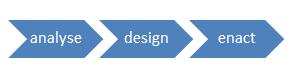
\includegraphics[width=.5\textwidth]{graphics/ade}
\end{center}

ADE minder i høj grad om traditionel software udvikling, idet der forsøges at planlægges og designes således der vil forekomme færre uforudsete problemer.

I modsætning til ADE vil CDA ikke forudsige, men nærmere forsøge at kontrollere.
Dette er en iterativ proces, i stil med agil software udvikling:\\
\begin{center}
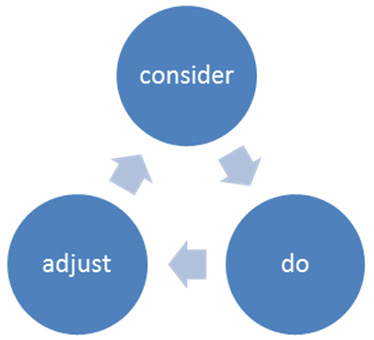
\includegraphics[width=.5\textwidth]{graphics/cda}
\end{center}

Som \citet{rose2012software} nævner vil de fleste organisationer falde under begge paradigmer.
Dette ser vi umiddelbart også som værende tilfældet for vores forretning, hvorfor vi systematisk vil gennemgå sammenligningstabellen i \citet[p. 38]{rose2012software}.

\paragraph{Process:}I første omgang vil der vælges en sekventiel tilgang, da vi har hardware og software der skal laves og begge disse er meget sikkerhedskritiske.
Det menes derfor at det kunne være kritisk at få et ufærdigt produkt ud, da tilliden til vores forretning er vigtig.
Efter første udrulning vil der derimod kunne indføres en mere iterativ tilgang, når først vi har vundet den tillid.

\paragraph{Understanding of future:}
Vi vil gerne styre fremtiden, altså sætte en høj standard for sikkerhed som andre vil få svært ved at følge.
På denne måde skal vi være gode til at tilpasse os, så vores produkt følger med til de stigende/ændrede generelle sikkerhedskrav.

\paragraph{Attitude to market:} Vores produkt er som sådan ikke nyt, da der allerede findes adskillige måder at håndtere passwords og deling af passwords.
Vi forsøger derimod at skabe et nyt marked, ved at bringe et kombineret sikkerhedsprodukt til virksomheder, hvor de måske ikke er klar over at de har brug for det.

\paragraph{Attitude to technology development:}
Vi vil gerne være foran de andre, så vi kan sætte standarden for hvad god sikkerhed og så vi er de eneste der kan levere det optimalt.

\paragraph{Role of business planning:} Vi har ikke råd til fejl her, da hvis vi først får leveret en dårlig løsning, vil vores (potentielle) kunder få svært ved at have tillid til os efterfølgende.
Derfor vil vi gerne ramme vores segment meget præcist, således at vi kan levere det bedst mulige produkt.

\paragraph{Software development style:} Agile og lean, da vi gerne vil have et velafprøvet og veltestet produkt.
Usability er igen vigtigt, da vi gerne vil have vores produkt så problemfrit integreret som muligt.

\paragraph{Attitude to change:}
Vi prøver at skabe et nyt marked, så vi ser ændringer som muligheder for at lave et bedre og mere fleksibelt produkt.

\paragraph{Funding approach:} Venture capital, så vi kan få sikret kvalitet inden produktet frigives, sådan at vores kunder ikke mister tilliden til os, ved en for dårlig tidlig løsning.

\paragraph{Approach to others working in the same areas:} Samarbejde er godt.
Hvis vi kan undgå at opfinde/lave alting selv er det en fordel.
Så kan vi udnytte andres erfaringer, sammenflette idéer og sælge dem videre som pakkeløsning.
Vores produkt er som sagt ikke nyskabende, vi prøver blot at samle tidligere løsninger og sælge dem til et nyt marked.

\paragraph{Approach to intellectual property:} Platformen er lukket, men de enkelte dele er åbne.
Vi prøver ikke at opfinde noget nyt, men prøver derimod at skabe en platform til bedre at udnytte de eksisterende teknologier i det nyskabte marked.

\paragraph{Partnering and Networking:} Netværk og samarbejde er godt, samme som ovenover.

\paragraph{Time to market:} Se `Funding approach'.

\subsection{Outline phases or activities in the Business Model Design Process}
I følge \citet[pp. 244-259]{osterwalder2009business} er der et forslag til en anvendelig proces til når der skal udarbejdes en ny BM.
Her beskrives 5 faser: Mobilize, Understand, Design, Implement og Manage -- hvor hver fase består af en række aktiviteter der kan udføres for at opnå målene for de enkelte faser.
Undervejs vil der blive både udarbejdet og indført en BM, som til sidst vil blive vedligeholdt.
Den overordnede idé med dette er at det er svært at designe en BM, men lige så snart dette er gjort er det nemt at udføre denne.
Dette er en design-orienteret tilgang, i modsætning til en beslutnings-orienteret tilgang som derimod siger at det er nemt at finde på idéer og problemet ligger derimod i at vælge en af disse.

For at lave en (ny) BM for vores forretning, har vi fulgt de fem faser fra \citet[pp. 244-259]{osterwalder2009business}.
For hver fase har vi valgt de aktiviteter vi mener er relevante at nævne ifm. udviklingen af vores BM.

\subsubsection{Mobilize}
\paragraph{Test preliminary business ideas}
Vores BM diskuteres internt, på tværs af hele organisationen, da denne ikke er så stor.
Det er vigtigt at udviklere, sikkerhedsekspert, usability-ekspert og sælgere har en fælles forståelse og enighed omkring forretningens BM.

\paragraph{Assemble team}
Som blev nævnt i \cref{resource-based} og \cref{value_chain} er der samlet et hold.
Dette hold er alsidigt, således at en grundig evaluering af de initielle BMs kan foretages.
Her er det muligt for ethvert medlem af forretningen at bruge deres område/ekspertise til at evaluere de enkelte dele af forretningens BM.

\subsubsection{Understanding}
\paragraph{Study potential customers}
Vi vil undersøge vores potentielle kunder (virksomheder) og den måde hvorpå de håndtere sikkerheds nu.
Altså, hvilke sikkerhedsprotokoller har de, hvis nogen, og i så fald hvordan indkorporeres de i deres arbejdsproces.
Det er også vigtigt at vi fra starten af virker professionelle, så vi kan udvinde en tillid, som er vigtigt med så følsomt et område.

\paragraph{Interview experts}
Vi skal bruge vores sikkerhedsekspert og usability ekspert.
\paragraph{Research already tried}
Her kunne vi kigge på eksisterende løsninger (e.g. LastPass, 1Password) og se hvad de har gjort for at blive udbredte indenfor et marked der minder meget om vores eget.\stefan{Minder vores marked om deres? Eller et andet spørgsmål, hvad er deres marked?}

\subsubsection{Design}
\paragraph{Prototype}
Vi forestiller os et usability lab i vores egen bygning, som skal afspejle den løsning vi vil give vores kunder.
Det vil sige vi har brug for et eller flere rum hvor vores løsning skal bruges for at få adgang til rummene.
I de rum skal også være det system der skal bruges til at logge på, samt håndtere centralisering og deling af passwords.

\paragraph{Brainstormet og testet BMs}
For at få testet vores BMs udefra vil vi konsultere os med dem vi mener der ved mest indenfor skabelsen af BMs: Ivan Aaen og Steen Palle (eller anden venture capital investor).\stefan{Hvem kender vi ellers? . . .}

\subsubsection{Implement}
\paragraph{Communicate and involve}
Allerede i Mobilize var hele forretningen en del af udviklingen af nye BM idéer, så det samme gør sig gældende her.

\subsubsection{Manage}
Her gælder samme holdning som kan ses tidligere i denne sektion.\bruno{Hvorhenne? :)}


\section{Diskuter to papers}

\subsection{Sarasvathy, S. D. (2001)}
%!TEX root=../master.tex

Dette afsnit omhandler \citet{sarasvathy2001effectuation}.

Sarasvathy foreslår et alternativ til den klassiske kausale tankegang omkring dannelse af nye virksomheder.
Hvor man tidligere har haft et fokus på at forstå sine omgivelser, for bedre at kunne forudsige og reagere på ændringer, foreslår Sarasvathy \textit{effectuation}.
Effectuation går ud på at styre sine omgivelser og tage udgangspunkt i de resourcer man allerede har til rådighed.

Der findes 4 principper i Effectuation:
\begin{itemize}
  \item Affordable loss -- rather than expected returns
  \item Strategic alliances -- rather than competitive analyses
  \item Exploitation of contingencies -- rather than preexisting knowledge
  \item Control of an unpredictable future -- rather than prediction of an uncertain one
\end{itemize}

\subsubsection{Relation til vores forretning}
Sarasvathy sætter de to paradigmer, causation og effectuation, op ret firkantet.
Ikke nødvendigvis at en er bedre end den anden, men at de tjener hver deres formål afhængigt af hvilken type forretning man ønsker at starte/har startet.
I tilfælde af at man prøve at overtage et marked der allerede eksisterer eller tilbyde et produkt der allerede findes, passer causation bedst, da der allerede er megen viden tilgængelig, således man kan analysere sig frem til en god indgangsvinkel.
Hvis man derimod har et nyt produkt eller prøver at komme ind på et nyt markedssegment, passer effectuation bedre, da det er mindre begrænsende.
Som man ser i eksemplet med U-Haul er der risiko for at forretningen slet ikke kommer fra start, da det kan vurderes ud fra tidlig analyse at det ikke er bæredygtigt at starte forretningen.
Derfor bør man se på hvilke resourcer man har og gå på kompromis med de mål man vil nå, for at komme i gang.

Hvis man ser på vores valg af paradigme i \cref{paradigme} hælder vi mest til effectuation.
Den største forskel er at vi har valgt at gå med venture capital, da vi mener at det vil være svært at få et start produkt i høj nok kvalitet til at vi kan gå videre.
Hvis vi havde valgt en ren effectuation tilgang, havde vi enten startet med et tilpas småt produkt som vi kunne have dækket gennem egen finansiering, eller ved at have holdt det som et side-projekt til et andet job (evt. studie).
Vi kunne også have valgt at skrue ned for forventningerne og have tilbudt et andet produkt end det vi vil kalde den endelige SharePass løsning, men måske i stedet starte med at tilbyde andre services, såsom sikkerheds-konsultering, indtil vi har de nødvendige resourcer til den løsning vi gerne så.


\subsection{Er vores valg a paradigme teoretisk eller empirisk validt?}
\subsection{Relater concepter brugt til artiklerne fra kurset}


\section{Kraaijenbrink}
Arbejdet fra \citet{kraaijenbrink2012nature} kritiserer de seks dimensioner brugt til at sammenligne causation og effectuation.
Nøglepunktet er at \citet{sarasvathy2001effectuation} bruger pragmatisme til at argumentere for effectuation modellen.
Men Kraaijenbrink mener det er bedre at den pragmatiske model bliver brugt når mennesker foretager handlinger.
Kraaijenbrink viser dette ved at gennemgå de seks dimensioner og vise hvordan de er blevet simplificeret og tilpasset causation og effectuation sammenlignings processen.
Vi vil kortfattet give en definition af pragmatisme og derefter gennemgå de seks dimensioner og vise hvad vi har brugt det Kraaijenbrink har fundet til.

\subsection{Pragmatisme}
Den pragmatiske model er defineret af følgende tre betegnelser.
\begin{itemize}
\item \textbf{Situatedness} - mennesker opfatter verdenen som en liste af muligheder som afgør hvordan de kan udføre ting.
\item \textbf{Corporeality} - opfattelsen er afgrænset af ens egne egenskaber og viden.
\item \textbf{Sociality} - social interaktion har indflydelse på menneskers handlinger.
\end{itemize}
En god beskrivelse a de tre betegnelser fra \citet{kraaijenbrink2012nature}:
\begin{quote}
  \textit{``First, humans always perceive the world in terms of the possible actions they can take. Hence, they perceive the world as a set of alternative opportunities that allow them to do certain things while being constrained from doing other things. Second, in perceiving these opportunities, humans are facilitated and constrained by their own body – their own capabilities, skills, and existing knowledge. Humans have a perception of their own abilities and take this into consideration when judging the opportunities they face. Finally, being social creatures, humans are facilitated and constrained by others. Humans mutually influence and persuade one another to take particular actions and to refrain from taking other actions.''}
\end{quote}

\subsection{De seks dimensioner}
En kort beskrivelse af hver dimension og Kraaijenbrinks kritikpunkter efterfulgt af hvad vi har brugt det til.

\paragraph{Starting point}
Denne dimension omhandler hvordan man starter ud i et proejkt.
I causation ser man på hvad man gerne vil opnå(Ends are given).
I effectuation ser man på hvad man har til rådighed(Means are given).
Vi har kigget på hvad vi har til rådighed se \cref{resource-based} uden at det er direkte sammenlignelig med effectuation.

\paragraph{Assumptions on future}
Denne dimension omhandler hvordan man ser ud i fremtiden.
Causation mener man at hvis man kan forudsige hvad der sker fx på markedet giver det kontrol.
I Effectuation er det omvendt, hvis man kan kontrollere fremtiden har man ikke brug for at forudsige den.
Kraaijenbrink mener at dette burde være to do dimensioner og at en person der bruger causation eller effectuation kan vælge kontrol over at forudsige eller omvendt.
Han mener at man her tager en pragmatisk beslutning.
Vi har valgt at kontrollere fremtiden ved at sætte en høj standard for sikkerheden i produktet, se \cref{paradigme}.

\paragraph{Predisposition toward risk}
Denne dimension omhandler hvordan man omgåes økonomiske risici.
I causation gør man det ved at prøve at optimere og maksimere omsætningen.
I effectuation ser man på hvor meget kapital de involverede er villige til at miste.
Her mener Kraaijenbrink igen at den ene model udelukker ikke den anden.
Dvs. man kan vælge hvad der giver mest mening pragmatisk set.

\paragraph{Appropriate for}
Denne dimension beskæftiger sig med om hvorvidt et firma fokuserer på nye eller eksisterende produkter og markeder.
Causation er for eksisterende produkter og markeder og effectuation for nye produkter og markeder.
Kraaijenbrinks første kritikpunkt er at det fremgår ikke klart i \citet{sarasvathy2001effectuation} om hvorfor man ikke skulle kunne anvende effectuation på eksisterende markeder.
Det andet kritikpunkt er at effectuation typisk kun er brugbart i agil udvikling.
Da vores produkt som sådan ikke er nyt, men nærmere en kombination af eksisterende løsninger kigger vi efter nye markeder, se \cref{paradigme}.

\paragraph{Attitude toward outside firms}
Denne dimension omhandler hvordan et firma begår sig i forhold til andre firmaer.
Enten samarbejder man(effectuation) eller så er man i åben konkurrence(causation).
Kraaijenbrink mener at der er mange firmaer og at litteraturen peger på at man sagtens kan have begge dele på en gang.
Vi har valgt at sammenarbejde se \cref{paradigme}.

\paragraph{Type of model}
Denne dimension omhandler hvilket miljø produktet skal udvikles til.
Det er om det kan udvikles med en lineær proces(statisk miljø) eller en cyklisk proces(dynamisk miljø).
Igen mener Kraaijenbrink at det ene ikke udelukker det andet.
Vi har valgt agil udvikling fordi produktet skal være meget brugervenligt og skal så hvidt muligt ikke ændre arbejdsfremgangen hos virksomheder.


\printbibliography[heading=bibintoc]

\end{document}
